In this section, we present our roque switch and 

\subsection {OpenFlow Protocol}
OpenFlow is the protocol used to communicate between the controller and its switches. An OpenFlow packet header is simply an 8 byte packet with the first byte used to communicate version, the second byte for type, third and fourth byte for message length followed by a four byte Transaction ID (see Figure 1). The type is of a subset of 19 possible types, most of which are of type request (e.g. 16 = Stats Request) with the subsequent reply (e.g. 17 = Stats Reply). There are couple key point to note when dealing with the OpenFlow protocol. First, the transaction ID is used to correlate incoming OpenFlow messages with their appropriate responses much in the same way TCP uses SYN and ACK flags. For example, a features reply will (generally) not be accepted by the controller unless it contains the corresponding transaction ID from the features request. This protocol is also a two-way communication scheme and not simply switch replies to controller request. Several message types, to include packet input events, are switch initiated communications to the controller.  

\begin{figure}
  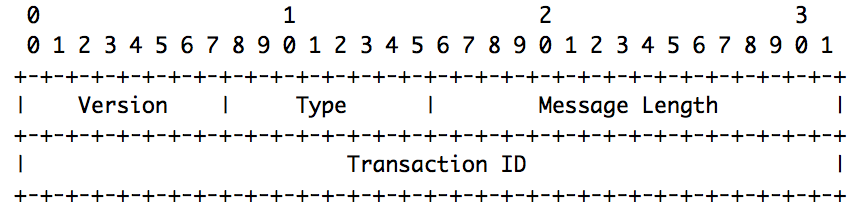
\includegraphics[width=\linewidth]{openflowProtocol.png}
  \caption{OpenFlow Protocol Header Format \cite{protocol}}
  \label{fig:protocol}
\end{figure}

\subsection {Controller Connection Sequence}
While the specific initiation sequence varies by controller , there are several required command to initiate a switch to controller connection\footnote{We specifically tested our roque switch on the Pox, Ryu and OpenDaylight controllers. Based on our testing and the OpenFlow specifications, we believe all controllers require this small subset of initialization commands but differences might exist based on implementation}. The switch to controller connection simply starts by opening a TCP connection to the controller on the configured port (default 6634)\footnote{As previously discussed, there is no authentication for this connection supported by any tested controller outside of certificate authentication only utilized with OpenVSwitch --- we need to verify that this statement is true. Only need to test our fakeswitch works outside of same box i.e. not only 127.0.0.1}.  After opening the connection, the switch sends a Openflow Hello message (0) to the controller. The controller then responds with a Hello message and a Features Request (5) message to which the switch responds with a  Features Reply (6). The controller then sends a Set Config message (9) that does not trigger a reply. Ryu follows this message with a Barrier Request (18), and OpenDaylight follows it with a  Get Config Request (7) to ensure switch configs are set appropriately. OpenDaylight also sends a Flow Modification message (14) to delete any previously installed flows on the switch.

The above commands are all that is needed for the initial controller to switch connection. The switch then proceeds to send several link layer neighbor discovery protocol messages as Packet Input Notification (10) messages to the controller including  Neighbor Solicitation and Router Solicitation messages. The switch also sends s Multicast Listener Report (part of the Multicast Listened Discovery Protocol Version 2) to the controller. Finally, the switch begins periodically (approximately every 3 seconds) sending an OpenFlow Echo Request (2) to the controller as a form of a keep alive with the controller.

\subsection{Our Rogue Switch Utility}
Our Roque Switch Utility mimics the initial connection sequence to a controller in order to facilitate testing of switch and controller vulnerabilities. Our roque switch utility does not handle the actual routing of traffic and is instead simply used to disrupt controller and switch traffic flow\footnote{A more advanced utility including routing is discussed in our additional attack section as well as our future work}. The bulk of our utility is a OpenFlow message parser that handles and appropriately responds to controller messages in the correct message format. These messages are generally hardcoded mimicked responses from previously captured live switch communication with minimal dynamic pieces (the transaction id is dynamically assigned for instance). 
